\begin{figure}[!ht]
    \centering
    \begin{minipage}[b]{0.45992852703\textwidth}
        \centering
        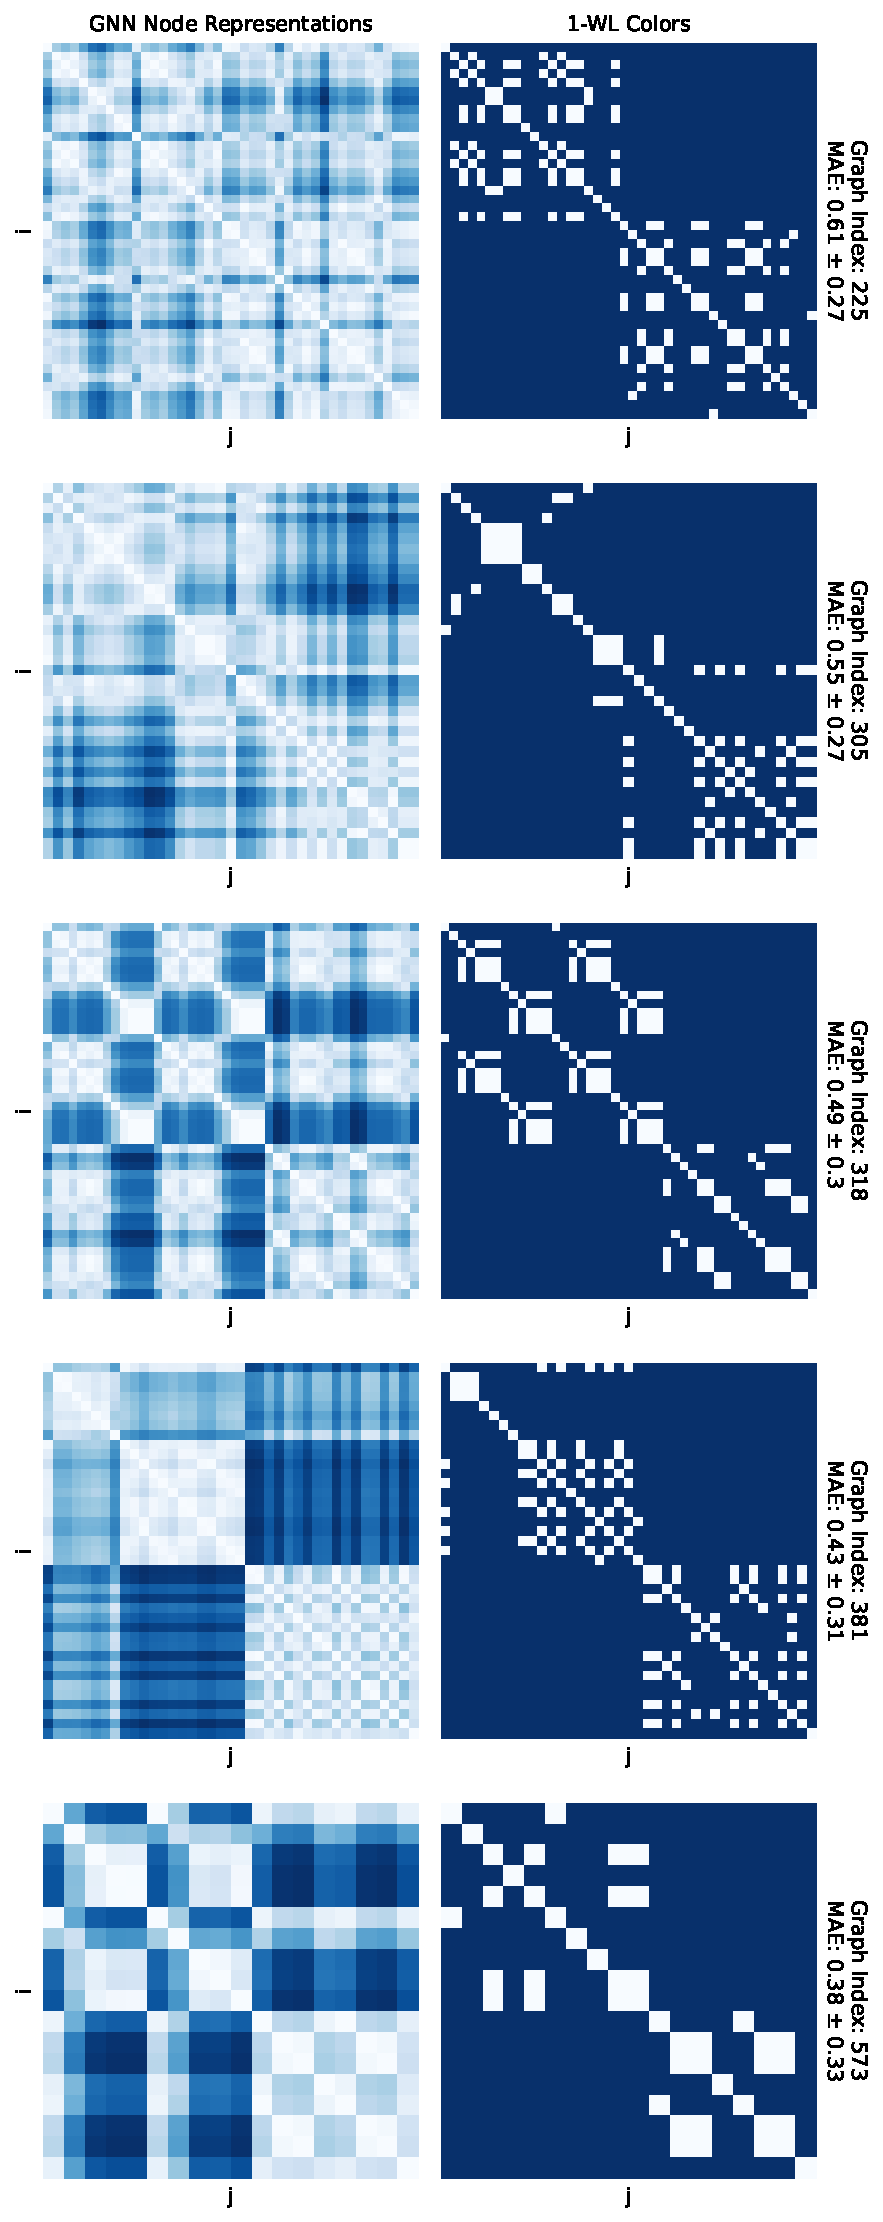
\includegraphics[width=\textwidth, left]{Figures/heatmaps_ENZYMES_0.pdf}
    \end{minipage}
    \hfill
    \begin{minipage}[b]{0.53007147296\textwidth}
        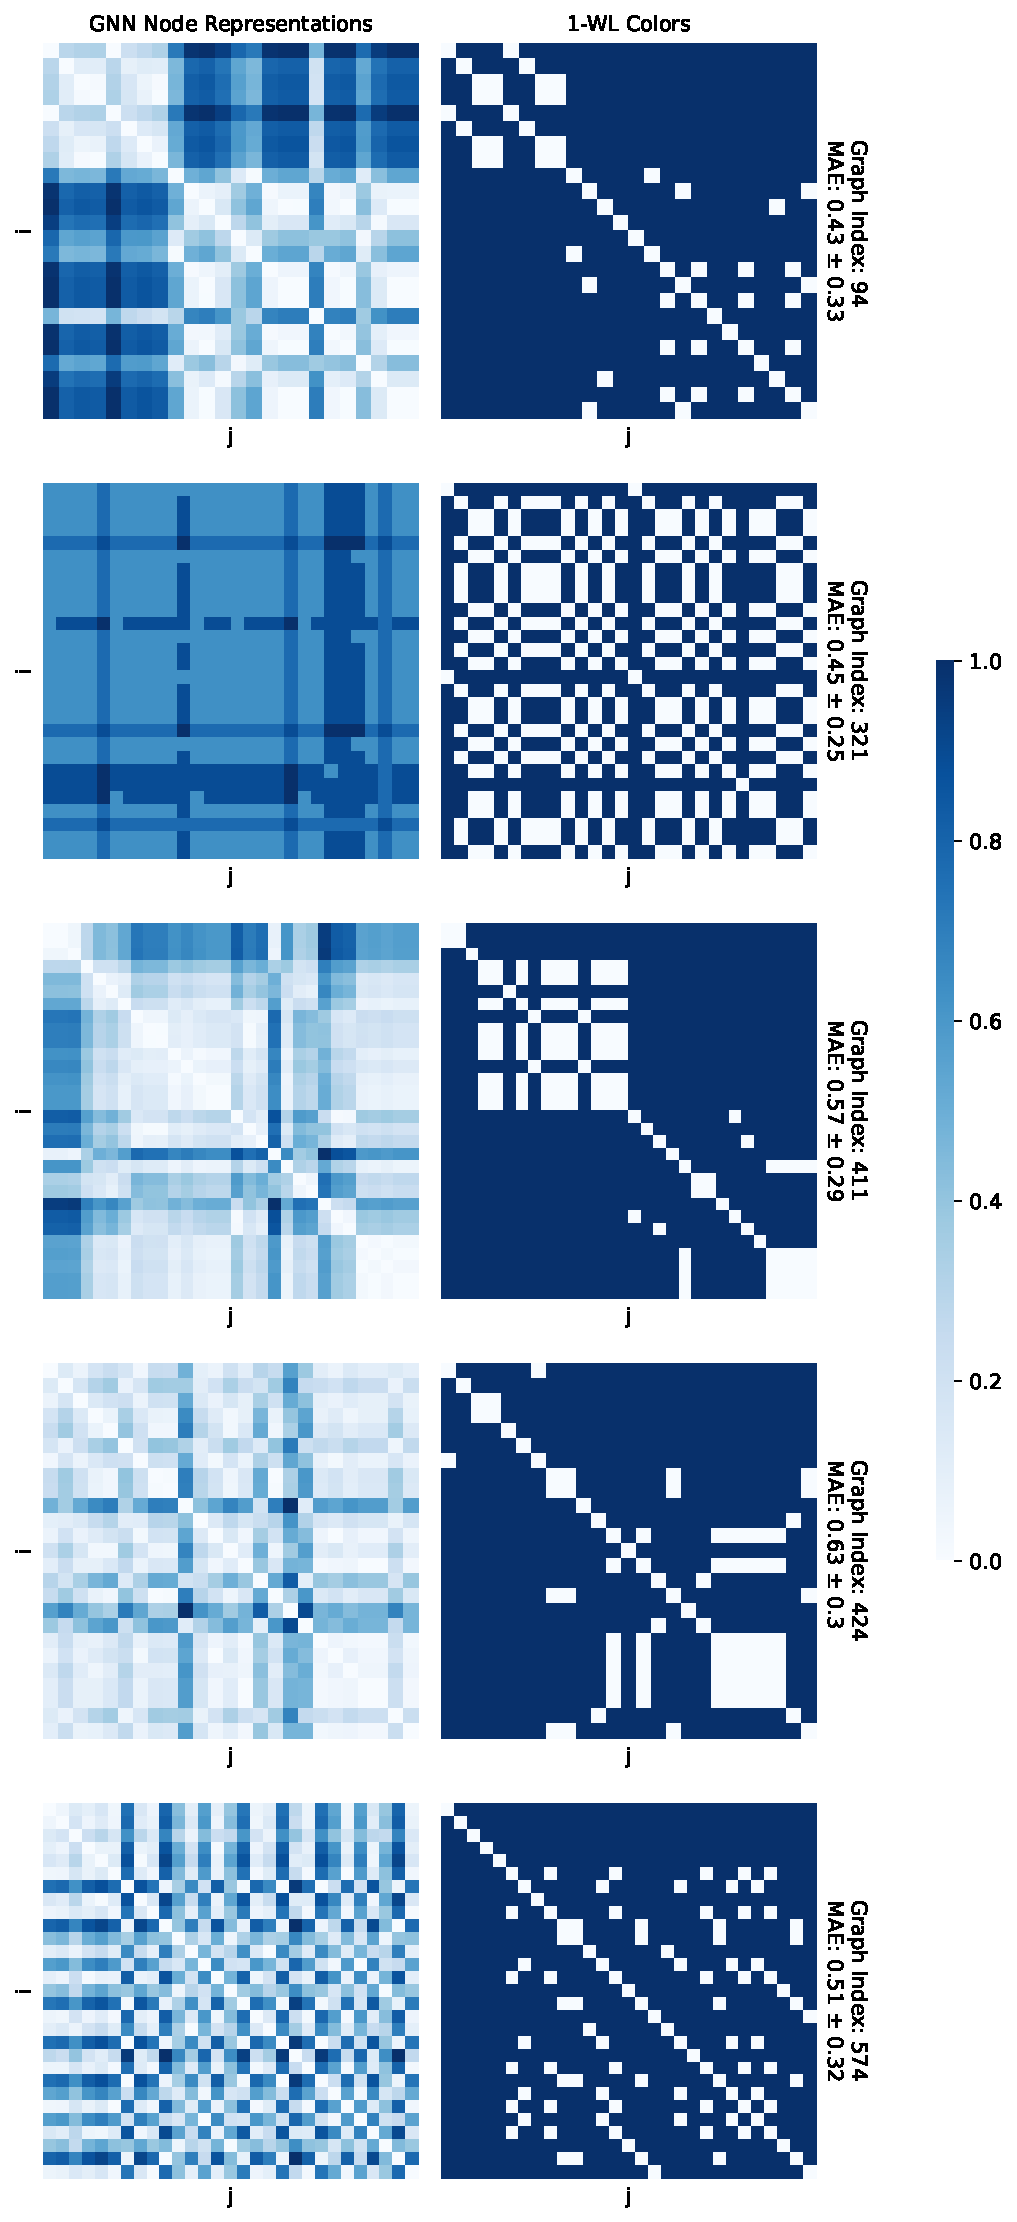
\includegraphics[width=\textwidth, right]{Figures/heatmaps_ENZYMES_1.pdf}
    \end{minipage}
    \hfill
    \caption{A visualization of 10 randomly sampled graphs, for how well the best performing GNN on dataset ENYZMES approximates the node colors computed by 1-WL algorithm with $1$ iteration. The average normalized error for the entire test set is: $0.49 ± 0.3$.}
\end{figure}

\begin{figure}[!ht]
    \centering
    \begin{minipage}[b]{0.45992852703\textwidth}
        \centering
        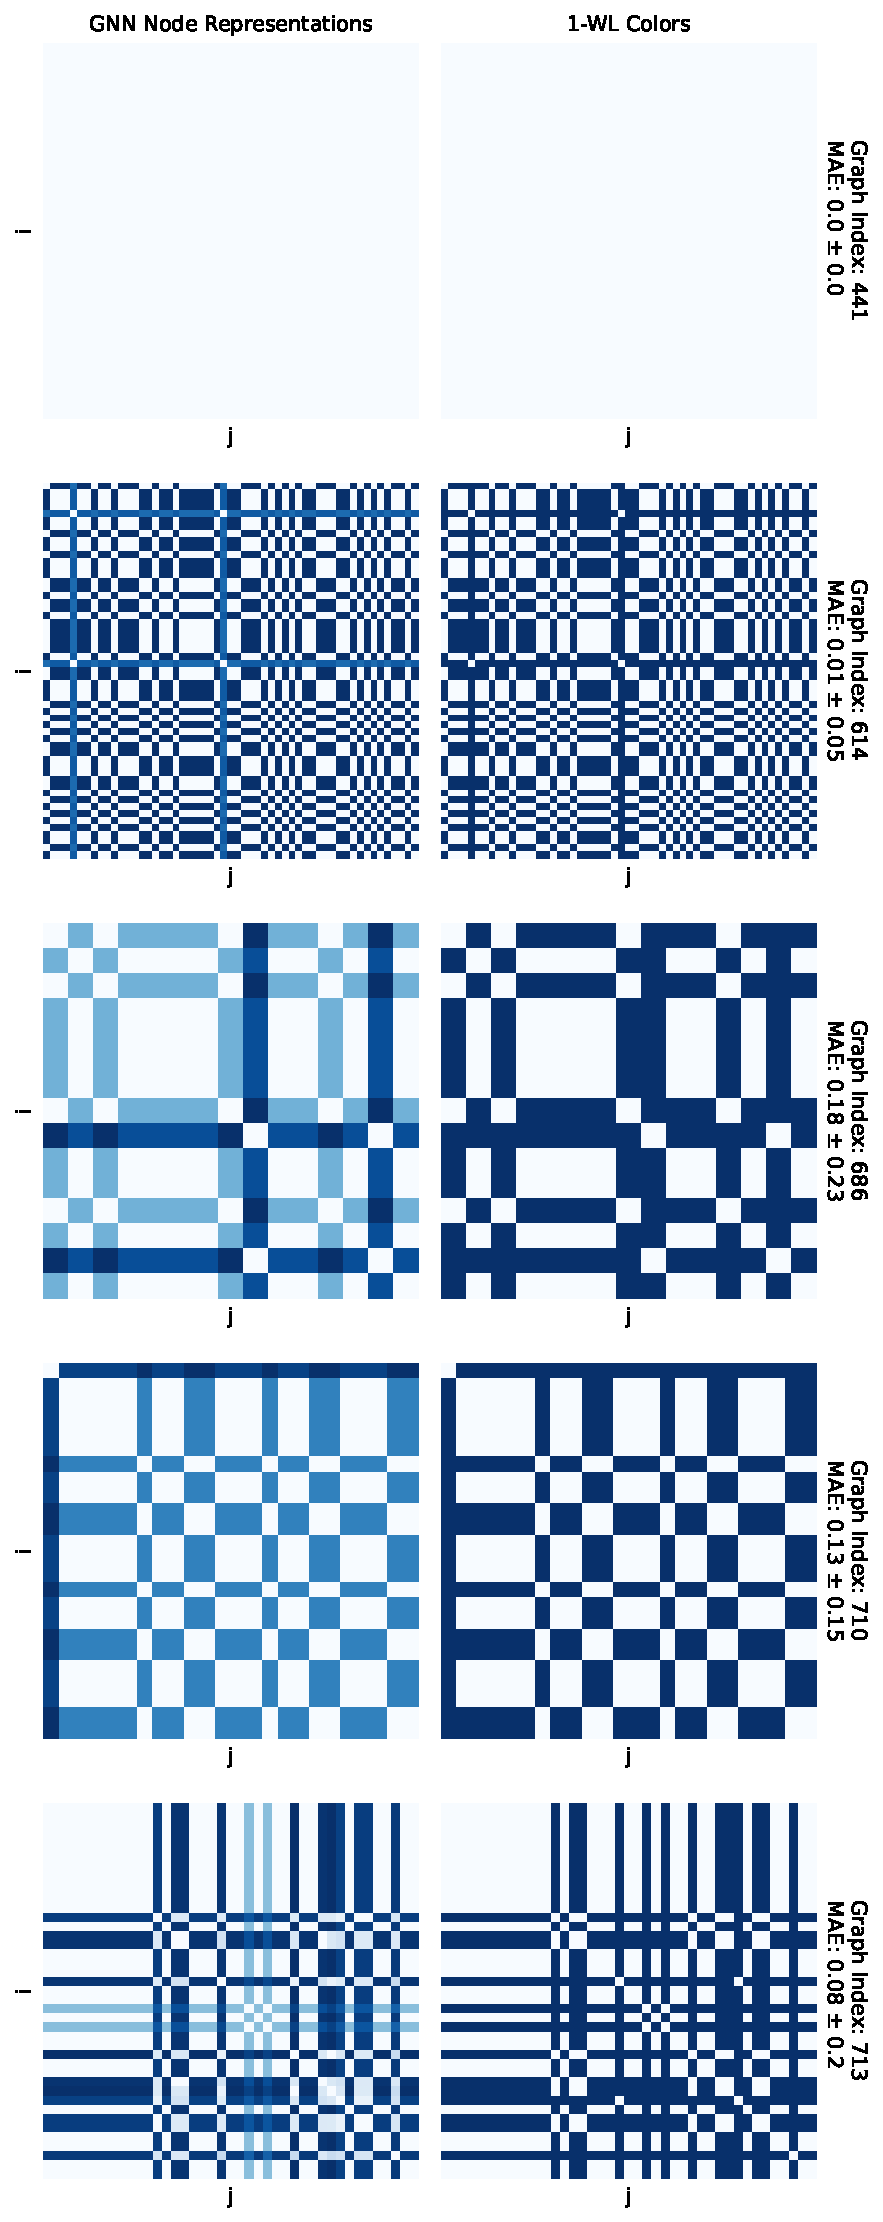
\includegraphics[width=\textwidth, left]{Figures/heatmaps_IMDB-BINARY_0.pdf}
    \end{minipage}
    \hfill
    \begin{minipage}[b]{0.53007147296\textwidth}
        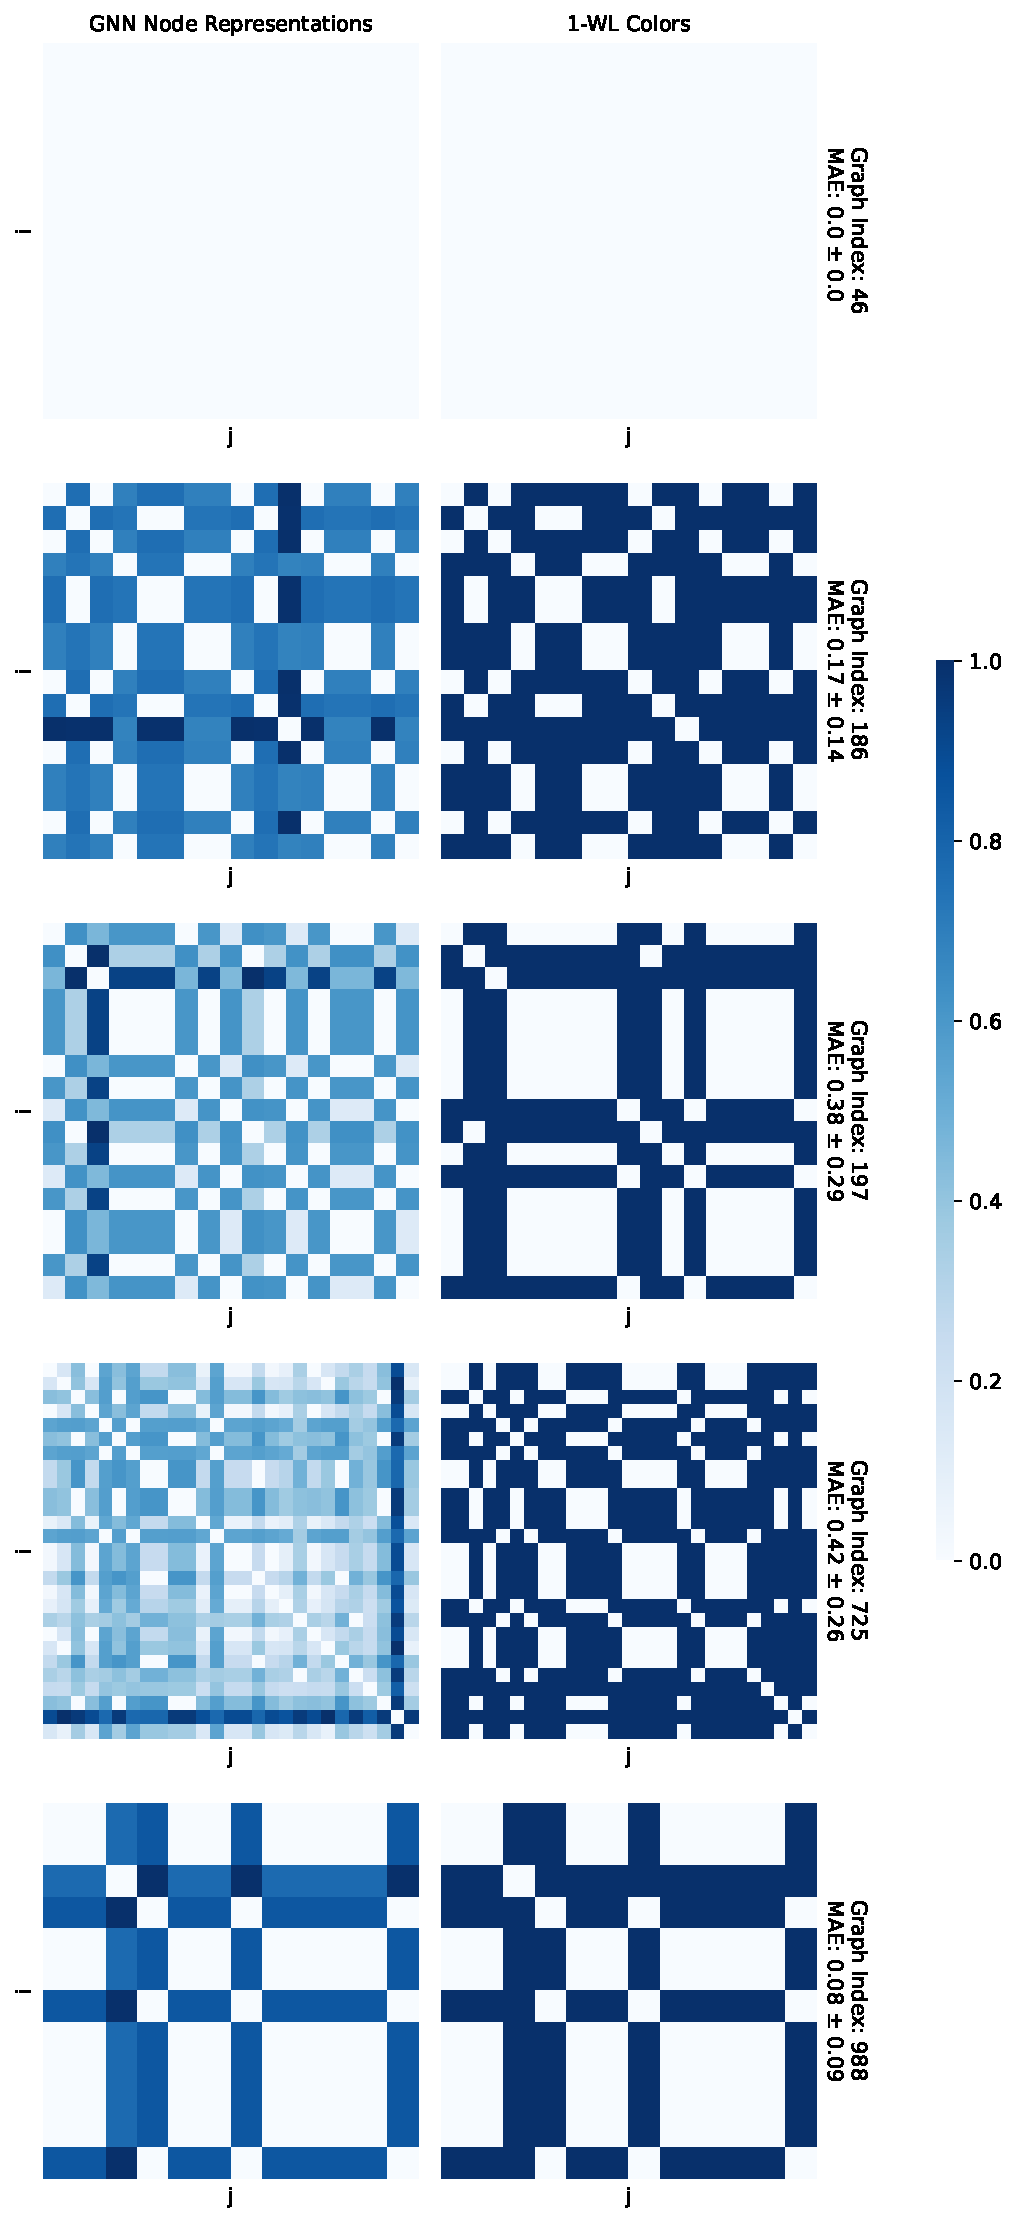
\includegraphics[width=\textwidth, right]{Figures/heatmaps_IMDB-BINARY_1.pdf}
    \end{minipage}
    \hfill
    \caption{A measure for evaluating the approximation performance of the 1-WL colors by the best performing GNN. The GNN was trained on the ENZYMES dataset, and the measure was applied to 10 randomly selected graphs from the GNN's test set. The average normalized error for the entire test set is: 0.14 ± 0.15.}
\end{figure}

\begin{figure}[!ht]
    \centering
    \begin{minipage}[b]{0.45992852703\textwidth}
        \centering
        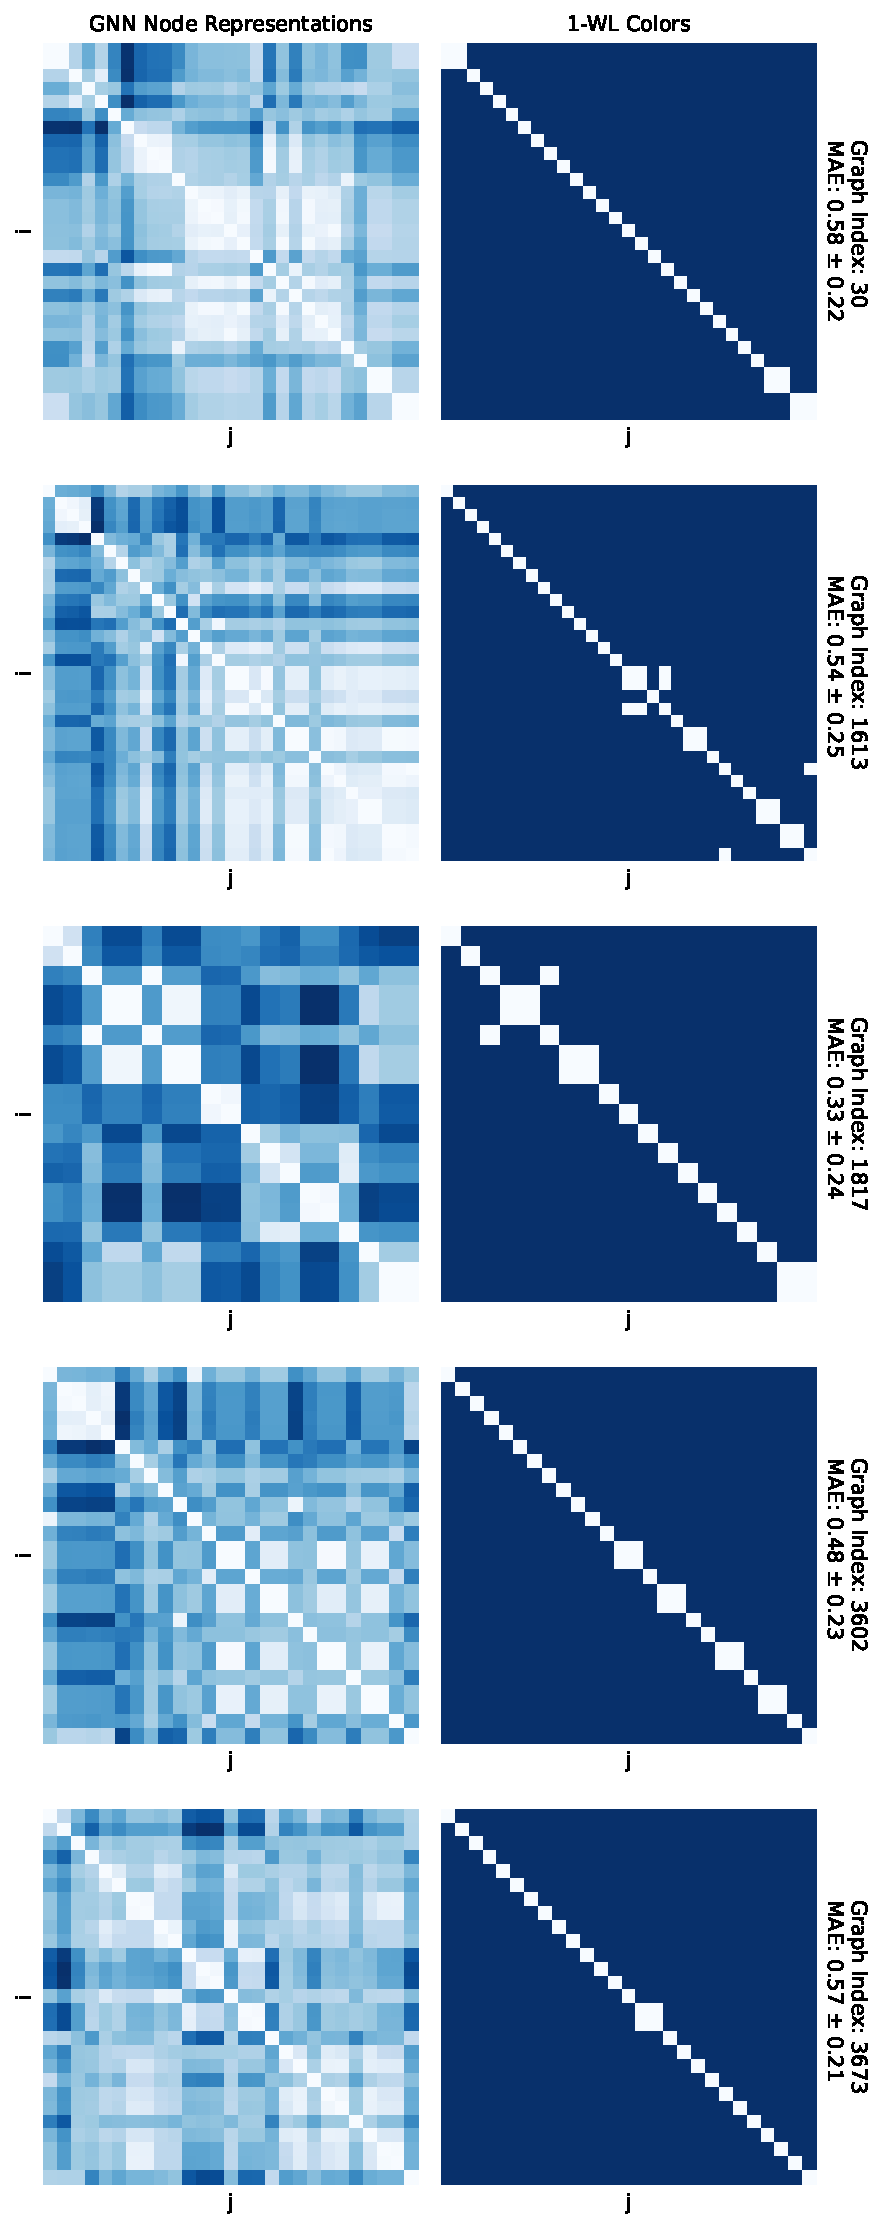
\includegraphics[width=\textwidth, left]{Figures/heatmaps_NCI1_0.pdf}
    \end{minipage}
    \hfill
    \begin{minipage}[b]{0.53007147296\textwidth}
        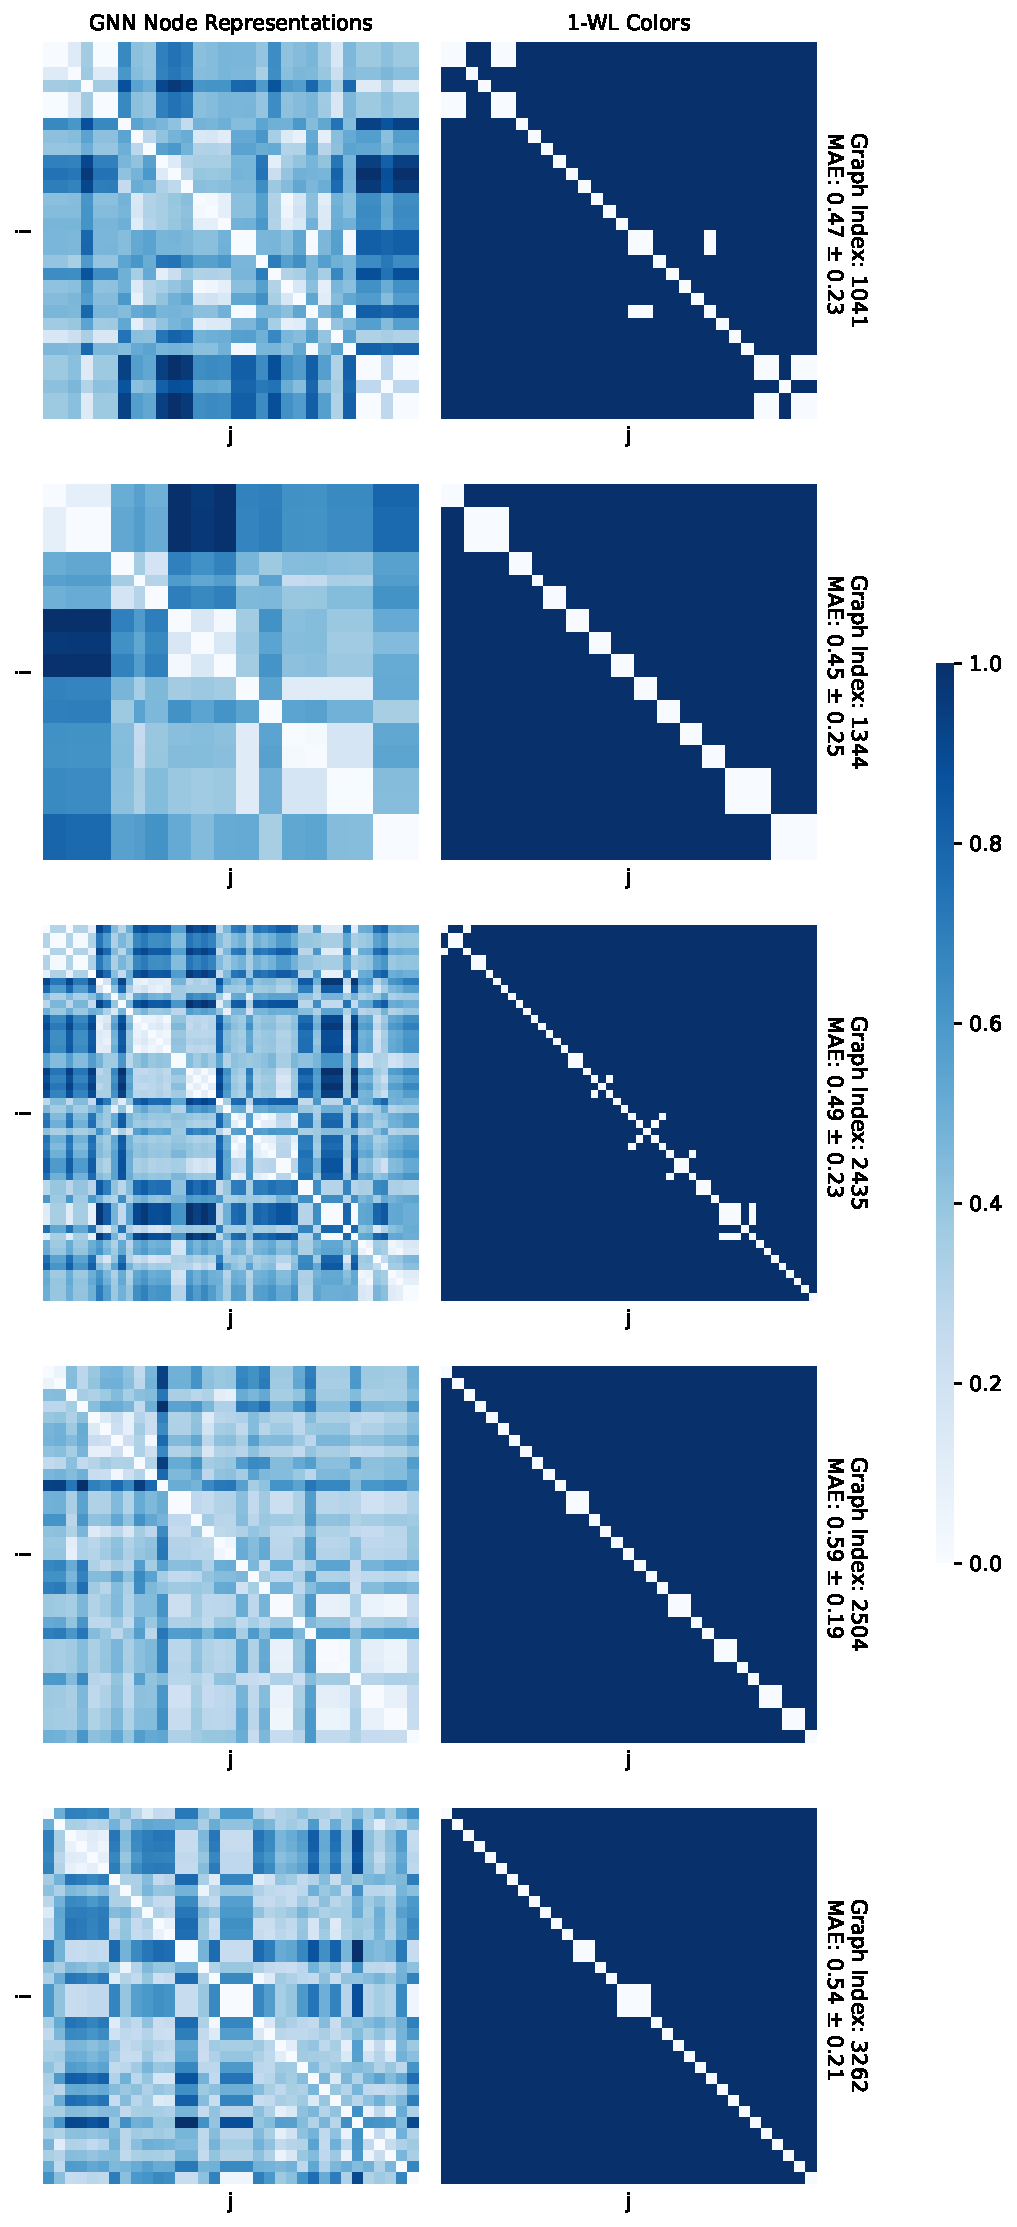
\includegraphics[width=\textwidth, right]{Figures/heatmaps_NCI1_1.pdf}
    \end{minipage}
    \hfill
    \caption{A measure for evaluating the approximation performance of the 1-WL colors by the best performing GNN. The GNN was trained on the ENZYMES dataset, and the measure was applied to 10 randomly selected graphs from the GNN's test set. The average normalized error for the entire test set is: 0.5 ± 0.24. k\_wl = 3}
\end{figure}

\begin{figure}[!ht]
    \centering
    \begin{minipage}[b]{0.45992852703\textwidth}
        \centering
        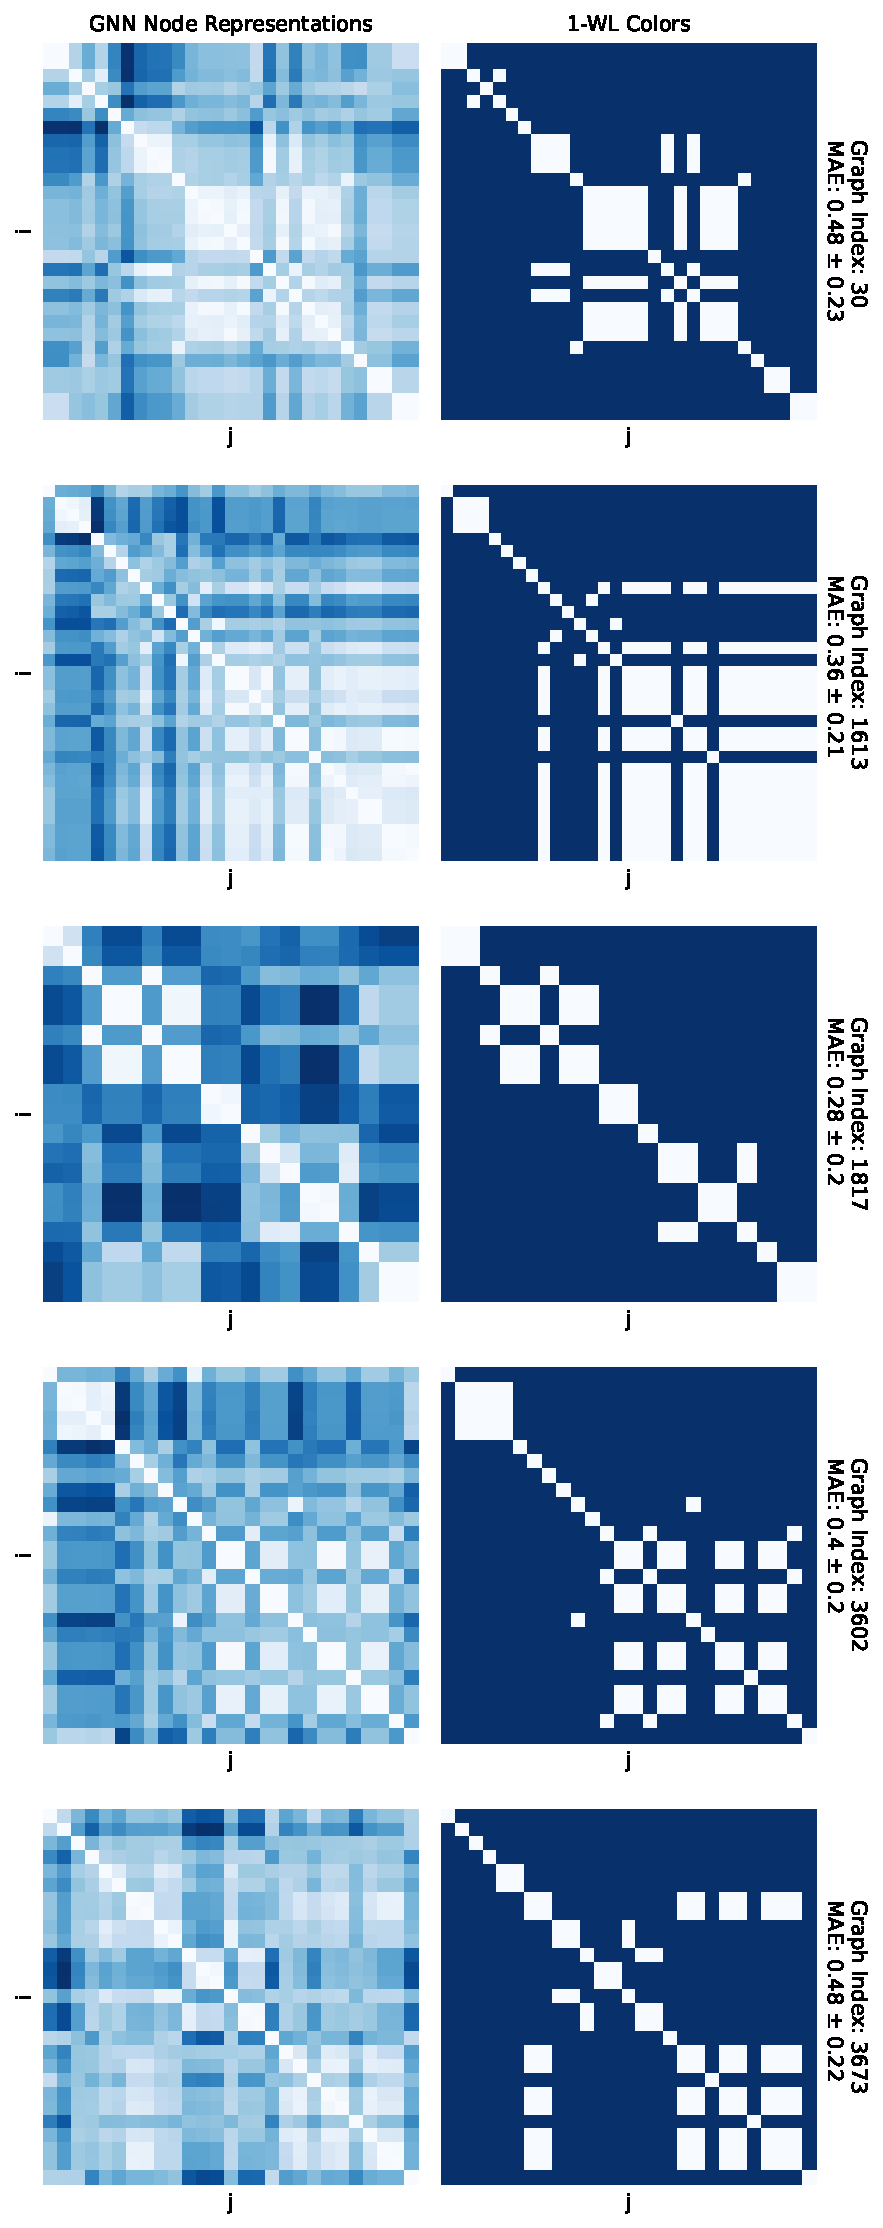
\includegraphics[width=\textwidth, left]{Figures/heatmaps_NCI1_0_k_wl_1.pdf}
    \end{minipage}
    \hfill
    \begin{minipage}[b]{0.53007147296\textwidth}
        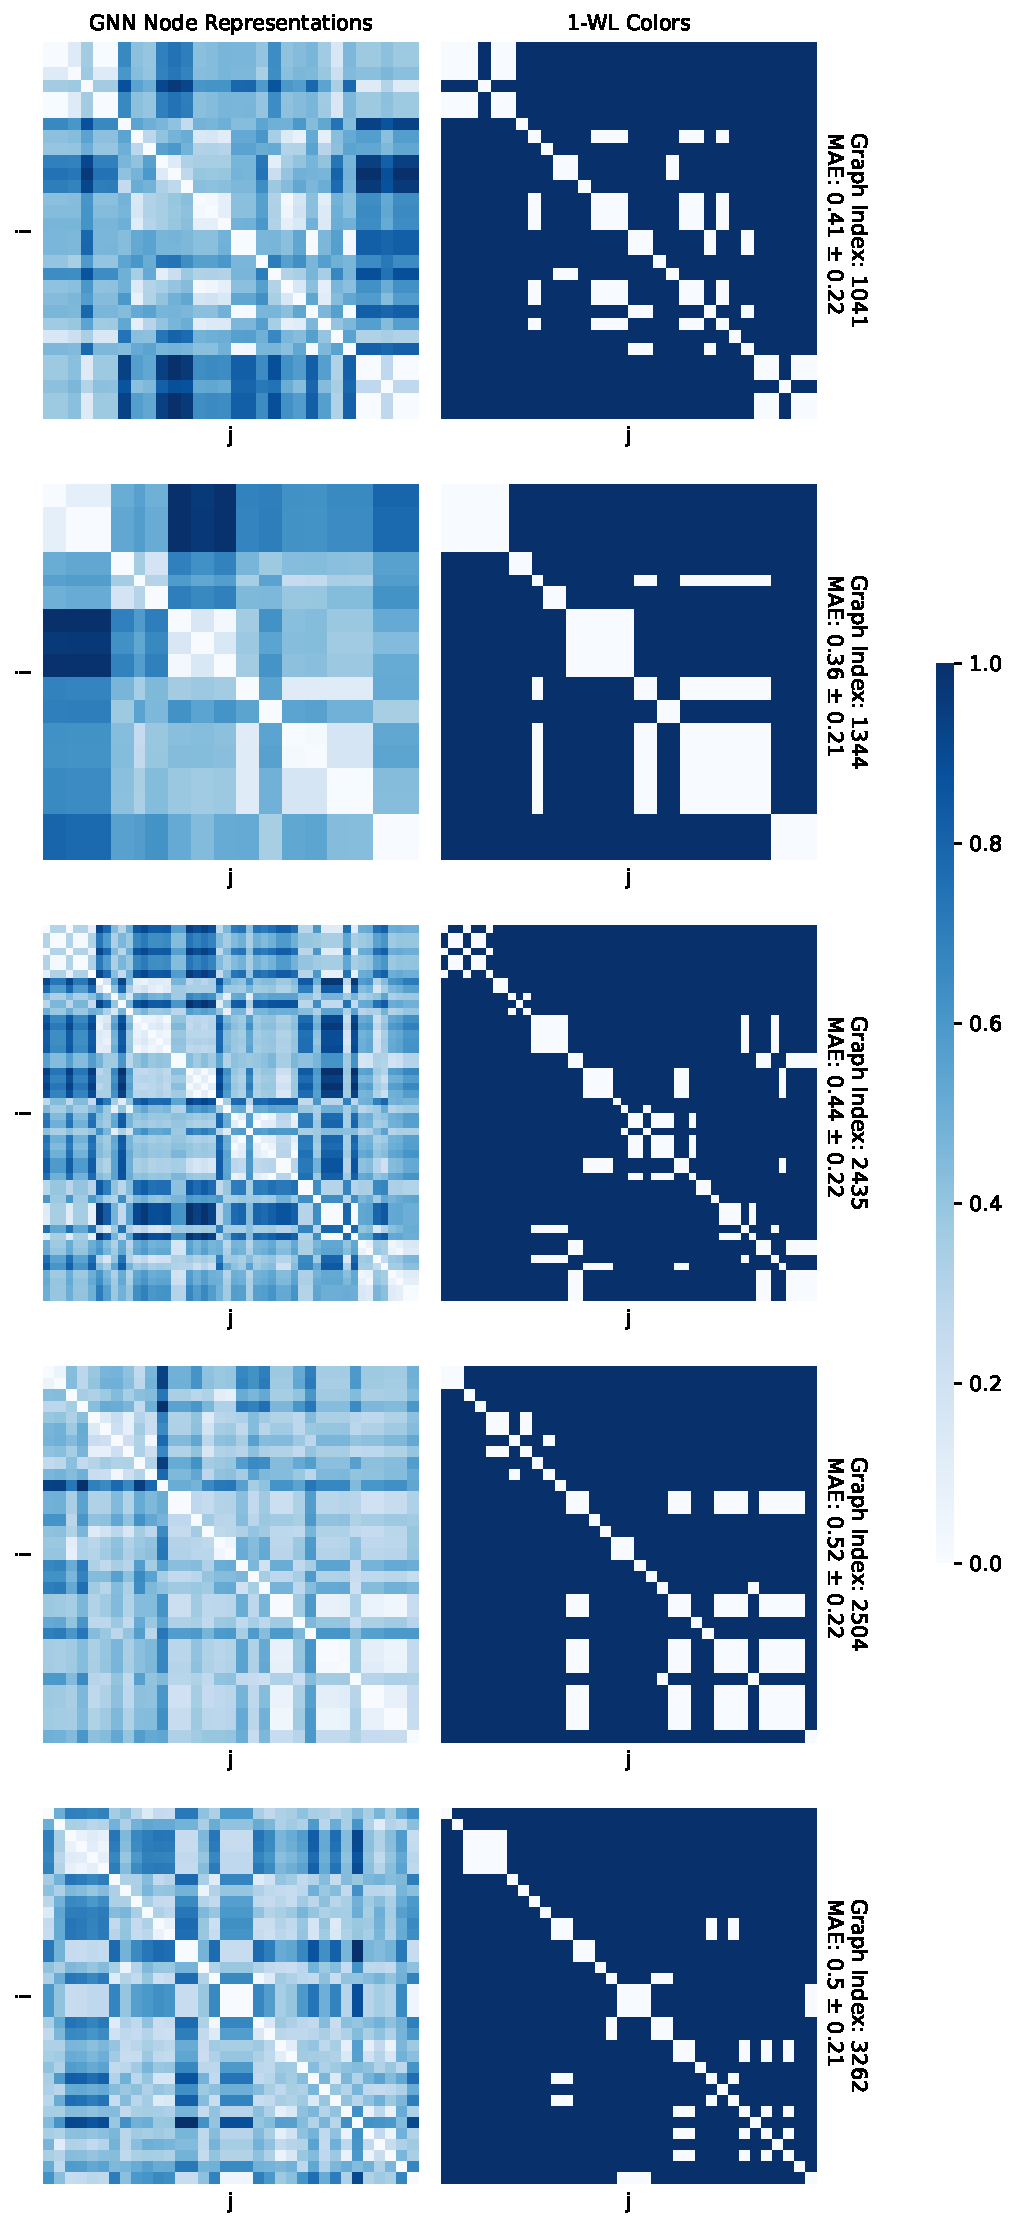
\includegraphics[width=\textwidth, right]{Figures/heatmaps_NCI1_1_k_wl_1.pdf}
    \end{minipage}
    \hfill
    \caption{A measure for evaluating the approximation performance of the 1-WL colors by the best performing GNN. The GNN was trained on the ENZYMES dataset, and the measure was applied to 10 randomly selected graphs from the GNN's test set. The average normalized error for the entire test set is: 0.42 ± 0.22, k\_wl = 1}
\end{figure}

\begin{figure}[!ht]
    \centering
    \begin{minipage}[b]{0.45992852703\textwidth}
        \centering
        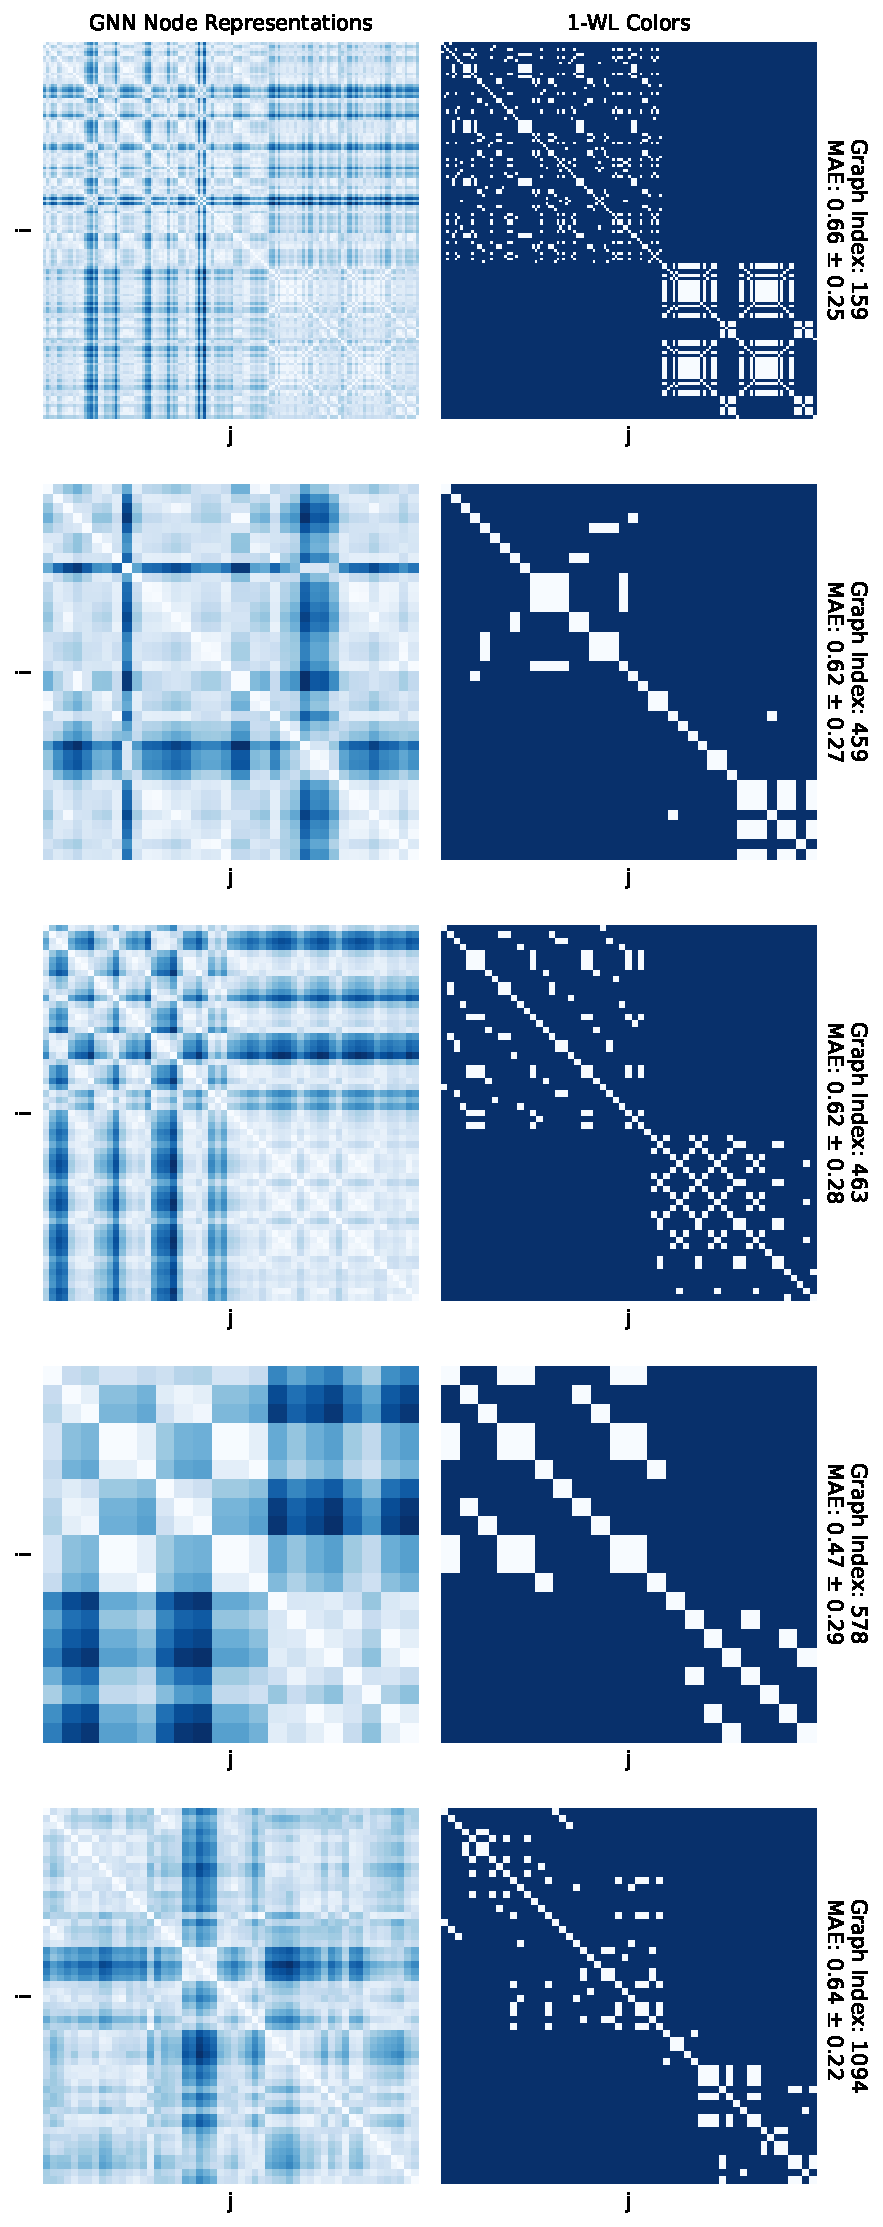
\includegraphics[width=\textwidth, left]{Figures/heatmaps_PROTEINS_0.pdf}
    \end{minipage}
    \hfill
    \begin{minipage}[b]{0.53007147296\textwidth}
        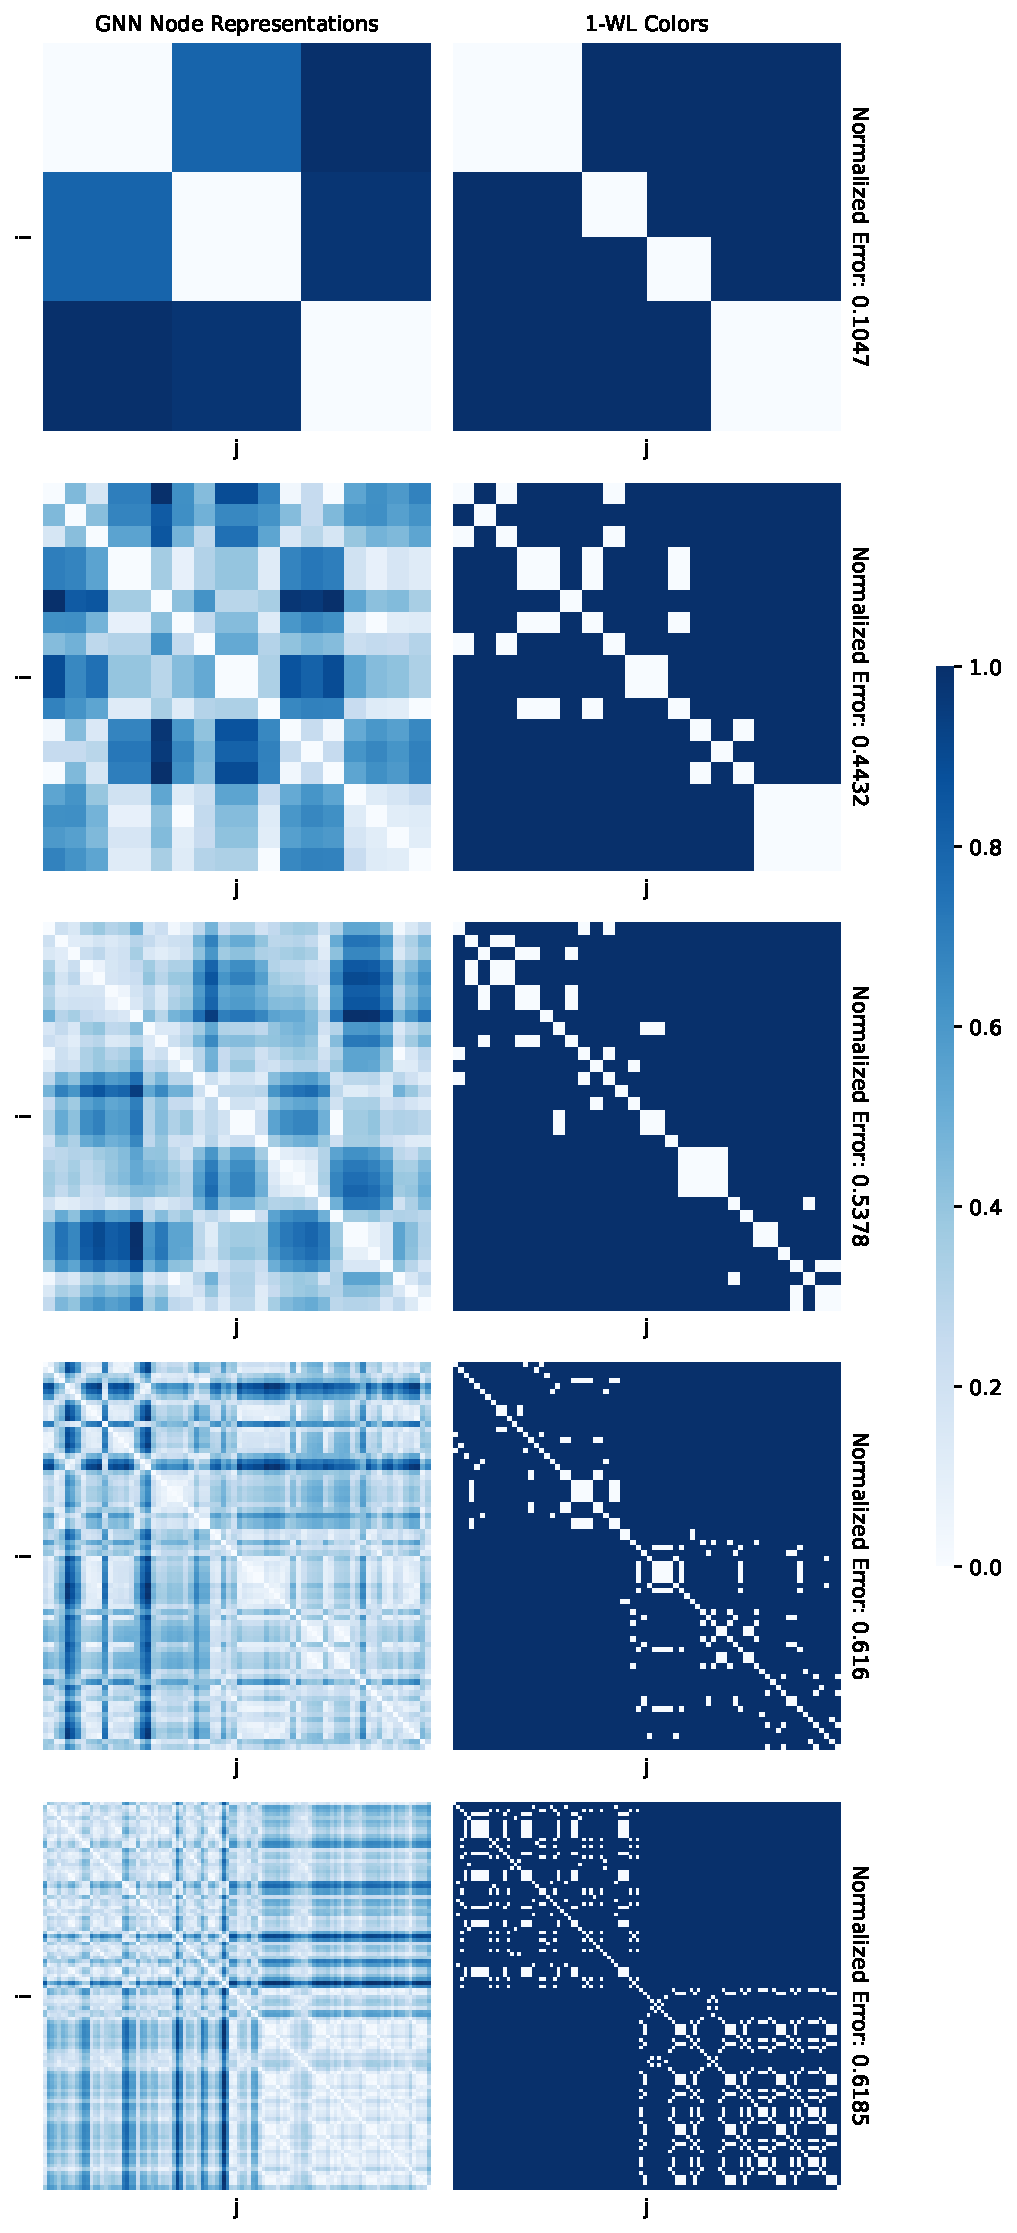
\includegraphics[width=\textwidth, right]{Figures/heatmaps_PROTEINS_1.pdf}
    \end{minipage}
    \hfill
    \caption{A measure for evaluating the approximation performance of the 1-WL colors by the best performing GNN. The GNN was trained on the ENZYMES dataset, and the measure was applied to 10 randomly selected graphs from the GNN's test set. The average normalized error for the entire test set is: 0.49 ± 0.26.}
\end{figure}